%%% Template originaly created by Karol Kozioł (mail@karol-koziol.net) and modified for ShareLaTeX use

\documentclass[a4paper,11pt]{article}

\usepackage[T1]{fontenc}
\usepackage[utf8]{inputenc}
\usepackage{graphicx}
\usepackage{subcaption}
\usepackage{xcolor}
\usepackage{stmaryrd}

% \renewcommand\familydefault{\sfdefault}
% \usepackage{tgheros}
% \usepackage[defaultmono]{droidmono}
\usepackage{mathrsfs}

\usepackage{amsmath,amssymb,amsthm,textcomp}
\usepackage{enumerate}
\usepackage{multicol}
\usepackage{tikz}
\usepackage{hyperref}

\usepackage{geometry}
\geometry{left=25mm,right=25mm,%
bindingoffset=0mm, top=20mm,bottom=20mm}


\setlength{\parskip}{1em}
%\linespread{1.3}

\newcommand{\linia}{\rule{\linewidth}{0.5pt}}

% % custom theorems if needed
% \newtheoremstyle{mytheor}
%     {1ex}{1ex}{\normalfont}{0pt}{\scshape}{.}{1ex}
%     {{\thmname{#1 }}{\thmnumber{#2}}{\thmnote{ (#3)}}}
%
% \theoremstyle{mytheor}
% \newtheorem{defi}{Definition}

% my own titles
\makeatletter
\renewcommand{\maketitle}{
\begin{center}
\vspace{2ex}
{\Large \textsc{\@title}}
\vspace{1ex}
\\
\linia\\
\@author \hfill \@date
\vspace{4ex}
\end{center}
}
\makeatother
%%%

% custom footers and headers
\usepackage{fancyhdr}
\pagestyle{fancy}
\lhead{}
\chead{}
\rhead{}
%\lfoot{Lógica Proposicional}
\cfoot{}
%\rfoot{página \thepage}
\renewcommand{\headrulewidth}{0pt}
\renewcommand{\footrulewidth}{0pt}
%

% code listing settings
\usepackage{listings}
\lstset{
    language=Python,
    basicstyle=\ttfamily\small,
    aboveskip={1.0\baselineskip},
    belowskip={1.0\baselineskip},
    columns=fixed,
    extendedchars=true,
    breaklines=true,
    tabsize=4,
    prebreak=\raisebox{0ex}[0ex][0ex]{\ensuremath{\hookleftarrow}},
    frame=lines,
    xleftmargin=2em,
    framexleftmargin=2em,
    showtabs=false,
    showspaces=false,
    showstringspaces=false,
    keywordstyle=\color[rgb]{0.627,0.126,0.941},
    commentstyle=\color[rgb]{0.133,0.545,0.133},
    stringstyle=\color[rgb]{01,0,0},
    numbers=left,
    numberstyle=\small,
    stepnumber=1,
    numbersep=5pt,
    captionpos=t,
    escapeinside={\%*}{*)}
}

%% SET THEORY %%

\usepackage{mathtools}
\usepackage{xparse}
\DeclarePairedDelimiterX\set[2]{\{}{\}}{\,#1 \;\delimsize\vert\; #2\,}

\newcommand{\eqdef}{\stackrel{\text{def}}{=}}

%% local labels in equations %%

\usepackage{xargs}

\makeatletter
  \newcommandx{\Label}[1][1={\arabic{equation}}]%
    {\refstepcounter{equation}(\theequation)~\ltx@label{{#1}} &&}
\makeatother

%% Proof trees %%

\usepackage{fitch}

\usepackage{etoolbox}
\let\bbordermatrix\bordermatrix
\patchcmd{\bbordermatrix}{8.75}{4.75}{}{}
\patchcmd{\bbordermatrix}{\left(}{\left[}{}{}
\patchcmd{\bbordermatrix}{\right)}{\right]}{}{}

%% circled question mark %%

\usepackage{tikz}
\newcommand*\circled[1]{\tikz[baseline=(char.base)]{
            \node[shape=circle,draw,inner sep=.7pt] (char) {\footnotesize #1};}}
\newcommand{\result}{\circled{?}}

%% Venn Diagrams %%

\usepackage{venndiagram}

%% LOGICAL SYMBOLS %%

\newcommand{\liff}{\leftrightarrow}
\DeclarePairedDelimiterX\FORALL[3]{(}{)}{\,\forall #1 : #2 : #3 \,}
\DeclarePairedDelimiterX\EXISTS[3]{(}{)}{\,\exists #1 : #2 : #3 \,}
\DeclarePairedDelimiterX\eval[1]{\llbracket}{\rrbracket}{#1}
\newcommand{\sem}[1]{\eval{#1}^{\model}}
\newcommand{\semv}[2]{\eval{#2}^{\model,#1}}
\newcommand{\model}{\mathfrak{M}}
\newcommand{\interpretation}{\mathscr{I}}
\DeclareMathOperator{\dom}{dom}
\DeclareMathOperator{\fun}{fun}
\DeclareMathOperator{\rel}{rel}

\DeclareRobustCommand{\svdots}{% s for `scaling'
  \vcenter{%
    \offinterlineskip
    \vspace{5pt}
    \hbox{.}
    \vskip0.25\normalbaselineskip
    \hbox{.}
    \vskip0.25\normalbaselineskip
    \hbox{.}%
  }%
}

%% COMPLETE BOX %%
\def\fillbox{\quad[\qquad]\quad}

%% NO INDENT %%

\setlength{\parindent}{0pt}

%%%% LOCALDEFS %%%%

\newcommand{\ambassador}{\mathsf{ambassador}_1}
\newcommand{\person}{\mathsf{person}_1}
\newcommand{\country}{\mathsf{country}_1}
\newcommand{\sentto}{\mathsf{sentto}_2}
\newcommand{\knight}{\mathsf{knight}_1}
\newcommand{\knave}{\mathsf{knave}_1}
\newcommand{\alice}{\mathsf{alice}}
\newcommand{\bob}{\mathsf{bob}}
\newcommand{\tom}{\mathsf{tom}}
\newcommand{\carl}{\mathsf{carl}}

%%%----------%%%----------%%%----------%%%----------%%%

\begin{document}

\title{Semántica}

%\author{Lógica Matemática Elemental (1934)}

\date{}

\maketitle

\vspace*{-1cm}

Considere el siguiente modelo:

\begin{figure}[ht]
	\begin{minipage}[b]{0.45\linewidth}
		\centering
		\begin{venndiagram2sets}[
				labelA={\tiny$\knight$},
				labelB={\tiny$\knave$},
				labelOnlyA={\footnotesize$\alice$},
				labelOnlyB={\footnotesize$\bob$}
			]
		\end{venndiagram2sets}
		%\caption{}
		%\label{}
	\end{minipage}
	\hspace{0.5cm}
	\begin{minipage}[b]{0.50\linewidth}
		\centering
		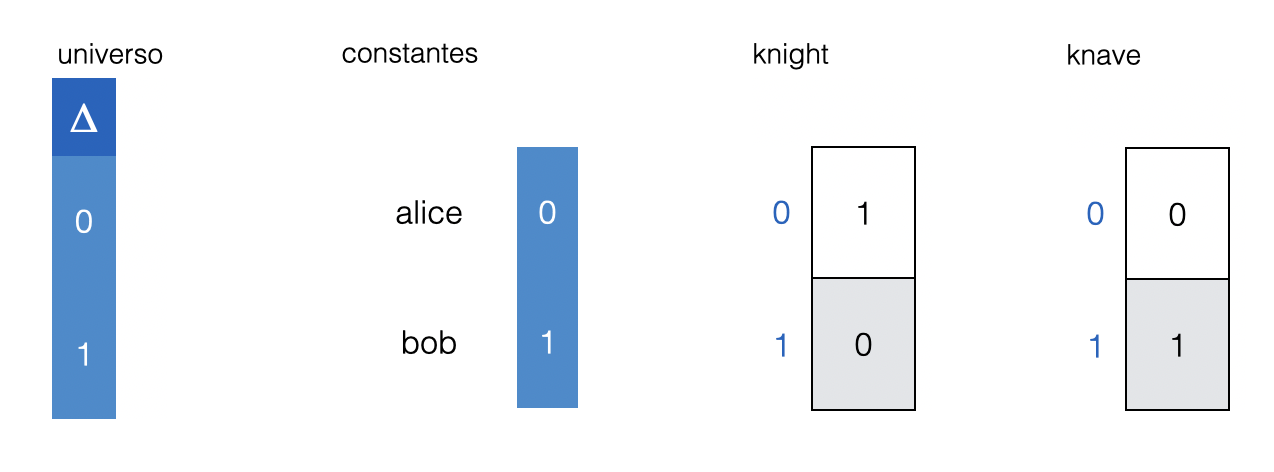
\includegraphics[width=\textwidth]{model1.png}
		%\caption{}
		%\label{}
	\end{minipage}
\end{figure}





\bigskip
{\bf valuación}
$\eval{\lnot \knight(\alice)} = 0$

{\bf justificación}

$
	\begin{nd}
		\hypo{}{\eval{\lnot \knight(\alice)}}
		\have{}{1 - \eval{\knight(\alice)}}

		\open
		\hypo{}{\eval{\knight(\alice)}}
		\have{}{1}
		\close
		\have{}{1-1}
		\have{}{0}
		\have{}{}

	\end{nd}
$

\newpage

Considere el siguiente modelo:

\begin{figure}[ht]
	\begin{minipage}[b]{0.45\linewidth}
		\centering
		\begin{venndiagram2sets}[
				labelA={\tiny$\knight$},
				labelB={\tiny$\knave$},
				labelOnlyB={\footnotesize$\alice$},
				labelOnlyA={\footnotesize$\bob$}
			]
		\end{venndiagram2sets}
		%\caption{}
		%\label{}
	\end{minipage}
	\hspace{0.5cm}
	\begin{minipage}[b]{0.45\linewidth}
		\centering
		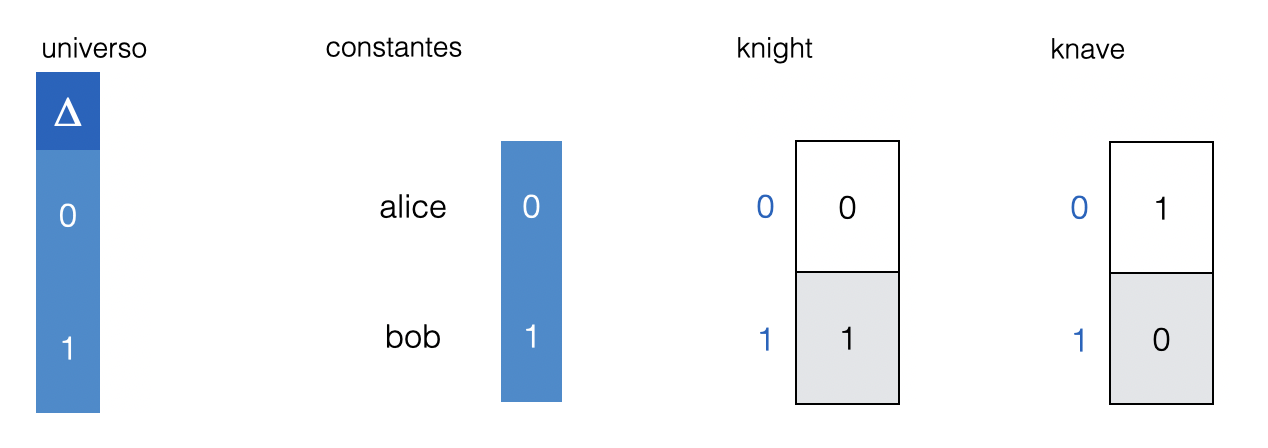
\includegraphics[width=\textwidth]{model3.png}
		%\caption{}
		%\label{}
	\end{minipage}
\end{figure}



\bigskip
{\bf valuación}
$\eval{\lnot \knight(\alice)} = 1$

{\bf justificación}

$
	\begin{nd}
		\hypo{}{\eval{\lnot \knight(\alice)}}
		\have{}{1 - \eval{\knight(\alice)}}
		\open
		\hypo{}{\eval{\knight(\alice)}}
		\have{}{0}
		\close
		\have{}{1-0}
		\have{}{1}
	\end{nd}
$

\newpage

Considere el siguiente modelo:


\begin{figure}[ht]
	\begin{minipage}[b]{0.45\linewidth}
		\centering
		\begin{venndiagram2sets}[
				labelA={\tiny$\knight$},
				labelB={\tiny$\knave$},
				labelOnlyA={\footnotesize$\alice$},
				labelOnlyB={\footnotesize$\bob$}
			]
		\end{venndiagram2sets}
		%\caption{}
		%\label{}
	\end{minipage}
	\hspace{0.5cm}
	\begin{minipage}[b]{0.50\linewidth}
		\centering
		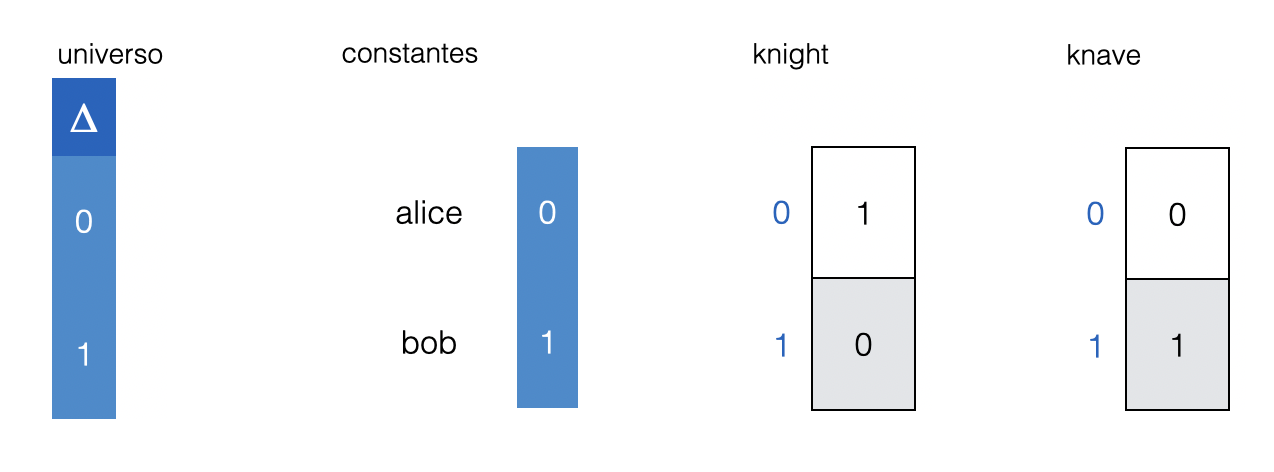
\includegraphics[width=\textwidth]{model1.png}
		%\caption{}
		%\label{}
	\end{minipage}
\end{figure}


\bigskip
{\bf valuación}
$\eval{\knight(\bob) \liff (\knight(\bob) \lor \knave(\alice))} = 1$

{\bf justificación}

$
	\begin{nd}
		\hypo{}{\eval{\knight(\bob) \liff (\knight(\bob) \lor \knave(\alice))}}
		\have{}{1-|\eval{\knight(\bob)} - \eval{(\knight(\bob) \lor \knave(\alice))}|}
		%\have{}{??}

		\open
		\hypo{}{\eval{\knight(\bob)}}
		\have{}{0}
		\close

		\open
		\hypo{}{\eval{(\knight(\bob) \lor \knave(\alice))}}
		\have{}{\max(\eval{\knight(\bob)}, \eval{\knave(\alice)})}
		\open
		\hypo{}{\eval{\knight(\bob)}}
		\have{}{0}
		\close
		\have{}{\eval{\knave(\alice)}}
		\have{}{0}
		\close
		\have{}{1 - |0 - 0|}
		\have{}{1}

	\end{nd}
$

\newpage
Considere el siguiente modelo:

\begin{figure}[ht]
	\begin{minipage}[b]{0.45\linewidth}
		\centering
		\begin{venndiagram2sets}[
				labelA={\tiny$\knight$},
				labelB={\tiny$\knave$},
				labelOnlyA={\footnotesize$\alice$},
				labelOnlyB={\footnotesize$\bob$}
			]
		\end{venndiagram2sets}
		%\caption{}
		%\label{}
	\end{minipage}
	\hspace{0.5cm}
	\begin{minipage}[b]{0.50\linewidth}
		\centering
		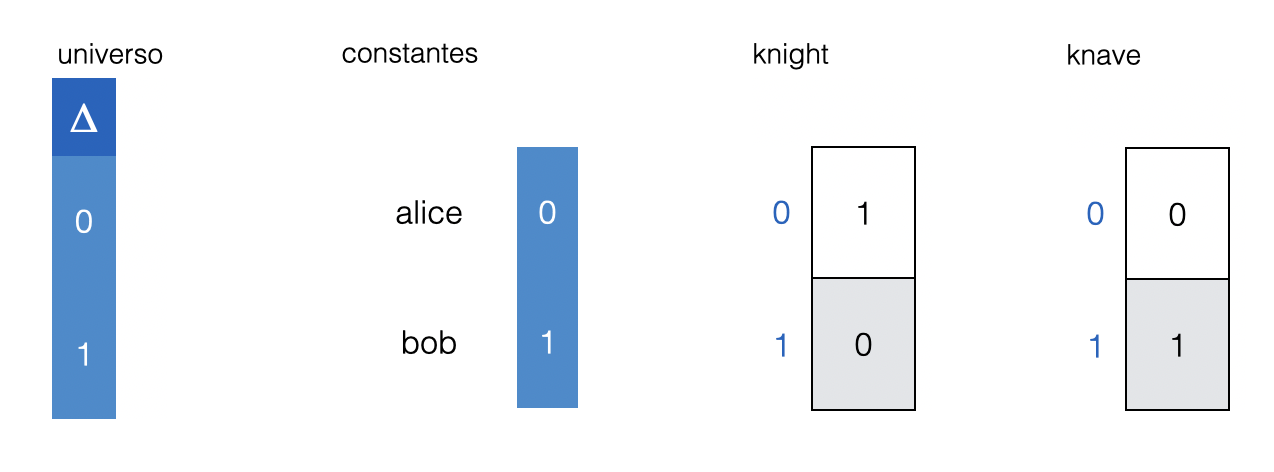
\includegraphics[width=\textwidth]{model1.png}
		%\caption{}
		%\label{}
	\end{minipage}
\end{figure}


\bigskip
{\bf valuación}
$\eval{\knight(\alice) \liff ((\knight(\alice) \land \knave(\bob)) \lor (\knave(\alice) \land \knight(\bob)))} = 1$

{\bf justificación}

$
	\begin{nd}
		\hypo{}{\eval{\knight(\alice) \liff ((\knight(\alice) \land \knave(\bob)) \lor (\knave(\alice) \land \knight(\bob)))}}
		\have{}{1 - |\eval{\knight(\alice)} - \eval{((\knight(\alice) \land \knave(\bob)) \lor (\knave(\alice) \land \knight(\bob)))}|}
		\open
		\hypo{}{\eval{\knight(\alice)}}
		\have{}{1}
		\close
		\open
		\hypo{}{\eval{((\knight(\alice) \land \knave(\bob)) \lor (\knave(\alice) \land \knight(\bob)))}}
		\have{}{\max(
			\eval{(\knight(\alice) \land \knave(\bob))},
			\eval{(\knave(\alice) \land \knight(\bob))})}
		\open
		\hypo{}{\eval{\knight(\alice) \land \knave(\bob)}}
		\have{}{\min(\eval{\knight(\alice)},\eval{\knave(\bob)})}
		\open
		\hypo{}{\eval{\knight(\alice)}}
		\have{}{1}
		\close
		\have{}{\eval{\knave(\bob)}}
		\have{}{1}
		\close
		\have{}{1}
		\close
		\have{}{1-|1-1|}
		\have{}{1}
	\end{nd}
$

\newpage
\begin{figure}[ht]
	\begin{minipage}[b]{0.45\linewidth}
		\centering
		\begin{venndiagram2sets}[
				labelA={\tiny$\knight$},
				labelB={\tiny$\knave$},
				labelOnlyA={\footnotesize$\alice$},
				labelOnlyB={\footnotesize$\bob$}

			]
		\end{venndiagram2sets}
		%\caption{}
		%\label{}
	\end{minipage}
	\hspace{0.5cm}
	\begin{minipage}[b]{0.50\linewidth}
		\centering
		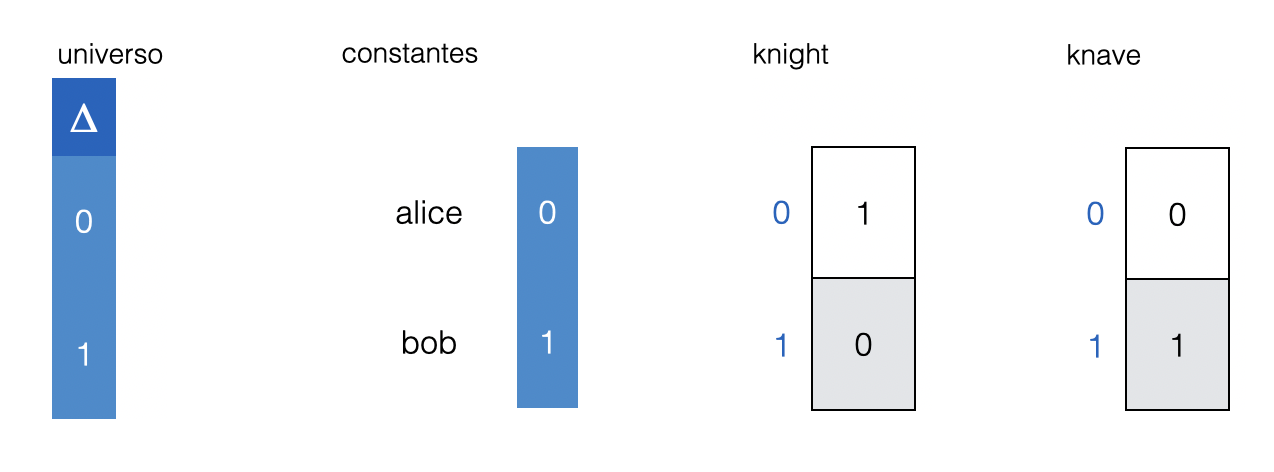
\includegraphics[width=\textwidth]{model1.png}
		%\caption{}
		%\label{}
	\end{minipage}
\end{figure}


{\bf valuación}
$\eval{(\forall x :: \knight(x))} = 0$

{\bf justificación}

$
	\begin{nd}
		\hypo{}{\eval{(\forall x :: \knight(x))}}
		\have{}{\min}
		% \open
		%     \hypo{}{\eval{\knight(x)} \text{~~cuando $x = 0$}}
		%     \have{}{1}
		% \close
		\open
		\hypo{}{\eval{\knight(x)} \text{~~cuando $x = 1$}}
		\have{}{0}
		\close
		%  \open
		%      \hypo{}{\eval{\knight(x)} \text{~~cuando $x = 2$}}
		%      \have{}{1}
		%  \close
		%  \open
		%      \hypo{}{\eval{\knight(x)} \text{~~cuando $x = 3$}}
		%      \have{}{0}
		%  \close
		%  \open

		%\hypo{}{\eval{\knight(x)} \text{~~cuando $x = 4$}}

		%\have{}{0}
		%\close
		%\open
		%    \hypo{}{\eval{\knight(x)} \text{~~cuando $x = 5$}}
		%    \have{}{1}
		%\close
		\have{}{0}
	\end{nd}
$

\newpage

\begin{figure}[ht]
	\begin{minipage}[b]{0.45\linewidth}
		\centering
		\begin{venndiagram2sets}[
				labelA={\tiny$\knight$},
				labelB={\tiny$\knave$},
				labelOnlyA={\footnotesize$0~~1~~5$},
				labelOnlyB={\footnotesize$2~~3~~4$}

			]
		\end{venndiagram2sets}
		%\caption{}
		%\label{}
	\end{minipage}
	\hspace{0.5cm}
	\begin{minipage}[b]{0.50\linewidth}
		\centering
		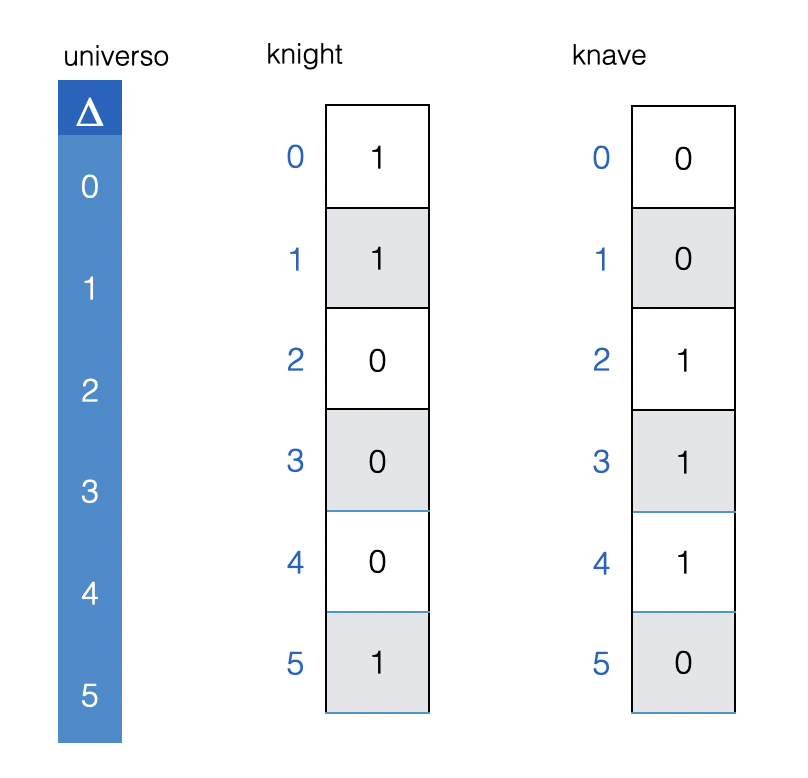
\includegraphics[width=\textwidth]{model4.png}
		%\caption{}
		%\label{}
	\end{minipage}
\end{figure}

{\bf valuación}
$\eval{(\forall x :: \knight(x) \lor \knave(x))} = 1$

{\bf justificación}

$
	\begin{nd}
		\hypo{}{\eval{(\forall x :: \knight(x) \lor \knave(x))}}
		\have{}{\min}
		\open
		\hypo{}{\eval{\knight(x) \lor \knave(x)} \text{~~cuando $x = 0$}}
		\have{}{\max(\eval{\knight(x)},\eval{\knave(x)})}
		\open
		\hypo{}{\eval{\knight(x)}}
		\have{}{1}
		\close
		\have{}{1}
		\close
		\open
		\hypo{}{\eval{\knight(x) \lor \knave(x)} \text{~~cuando $x = 1$}}
		\have{}{\max(\eval{\knight(x)},\eval{\knave(x)})}
		\open
		\hypo{}{\eval{\knight(x)}}
		\have{}{1}
		\close
		\have{}{1}
		\close
		\open
		\hypo{}{\eval{\knight(x) \lor \knave(x)} \text{~~cuando $x = 2$}}
		\have{}{\max(\eval{\knight(x)},\eval{\knave(x)})}
		\open
		\hypo{}{\eval{\knight(x)}}
		\have{}{0}
		\close
		\have{}{\eval{\knave(x)}}
		\have{}{1}
		\close
		\open
		\hypo{}{\eval{\knight(x) \lor \knave(x)} \text{~~cuando $x = 3$}}
		\have{}{\max(\eval{\knight(x)},\eval{\knave(x)})}
		\open
		\hypo{}{\eval{\knight(x)}}
		\have{}{0}
		\close
		\have{}{\eval{\knave(x)}}
		\have{}{1}
		\close
		\open
		\hypo{}{\eval{\knight(x) \lor \knave(x)} \text{~~cuando $x = 4$}}
		\have{}{\max(\eval{\knight(x)},\eval{\knave(x)})}
		\open
		\hypo{}{\eval{\knight(x)}}
		\have{}{0}
		\close
		\have{}{\eval{\knave(x)}}
		\have{}{1}
		\close
		\open
		\hypo{}{\eval{\knight(x) \lor \knave(x)} \text{~~cuando $x = 5$}}
		\have{}{\max(\eval{\knight(x)},\eval{\knave(x)})}
		\open
		\hypo{}{\eval{\knight(x)}}
		\have{}{1}
		\close
		\have{}{1}
		\close
		\have{}{1}
	\end{nd}
$

\newpage
{\bf valuación}
$\eval{(\forall x :: \knight(x) \lor \knave(x))} = 1$

{\bf justificación (agrupando)}

$
	\begin{nd}
		\hypo{}{\eval{(\forall x :: \knight(x) \lor \knave(x))}}
		\have{}{\min}
		\open
		\hypo{}{\eval{\knight(x) \lor \knave(x)} \text{~~cuando $x \in \{0,1,5\}$}}
		\have{}{\max(\eval{\knight(x)},\eval{\knave(x)})}
		\open
		\hypo{}{\eval{\knight(x)}}
		\have{}{1}
		\close
		\have{}{1}
		\close
		\open
		\hypo{}{\eval{\knight(x) \lor \knave(x)} \text{~~cuando $x \in \{2,3,4\}$}}
		\have{}{\max(\eval{\knight(x)},\eval{\knave(x)})}
		\open
		\hypo{}{\eval{\knight(x)}}
		\have{}{0}
		\close
		\have{}{\eval{\knave(x)}}
		\have{}{1}
		\close
		\have{}{1}
	\end{nd}
$

\newpage

\begin{figure}[ht]
	\begin{minipage}[b]{0.45\linewidth}
		\centering
		\begin{venndiagram2sets}[
				labelA={\tiny$\knight$},
				labelB={\tiny$\knave$},
				labelOnlyA={\footnotesize$\alice$},
				labelNotAB={\footnotesize$\bob$}

			]
		\end{venndiagram2sets}
		%\caption{}
		%\label{}
	\end{minipage}
	\hspace{0.5cm}
	\begin{minipage}[b]{0.50\linewidth}
		\centering
		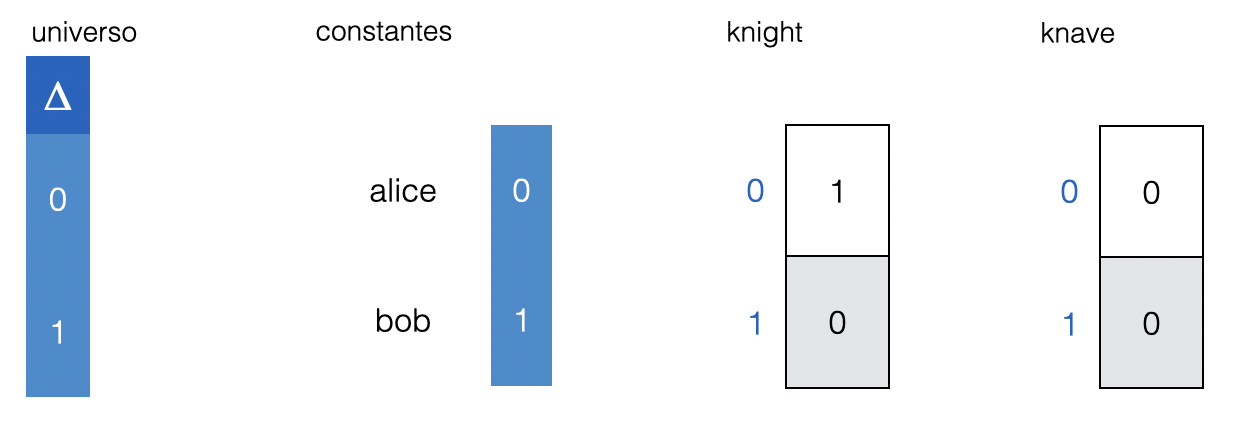
\includegraphics[width=\textwidth]{model5.png}
		%\caption{}
		%\label{}
	\end{minipage}
\end{figure}



{\bf valuación}
$\eval{(\forall x :: \knight(x) \lor \knave(x))} = ??$

{\bf justificación}

$
	\begin{nd}
		\hypo{}{\eval{(\forall x :: \knight(x) \lor \knave(x))}}
		\have{}{\min}
		\open
		\hypo{}{\eval{\knight(x) \lor \knave(x)} \text{~~cuando $x=1$}}
		\have{}{\max(\eval{\knight(x)},\eval{\knave(x)})}
		\open
		\hypo{}{\eval{\knight(x)}}
		\have{}{0}
		\close
		\have{}{\eval{\knave(x)}}
		\have{}{0}
		\close
		\have{}{0}
	\end{nd}
$

\newpage



%\begin{enumerate}
%    \item $\knight(\alice) \liff ((\knight(\alice) \land \knave(\bob)) \lor (\knave(\alice) \land \knight(\bob)))$
%    \item $\knight(\bob) \liff (\knight(bob) \lor \knave(\alice))$
%    \item $(\forall x :: \knight(x) \lor \knave(x))$
%    \item $\lnot(\exists x :: \knight(x) \land \knave(x))$
% \item $(\forall x :: \knight(x) \liff \lnot\knave(x))$
% \item $(\forall x :: \knight(x) \liff \lnot\knave(x)) \lor (\forall x :: \lnot\knight(x) \liff \knave(x))$
% \item $(\forall x :: (\knight(x) \liff \lnot\knave(x)) \lor (\lnot\knight(x) \liff \knave(x)))$
%\end{enumerate}

\newpage

\begin{figure}[ht]
	\begin{minipage}[b]{0.40\linewidth}
		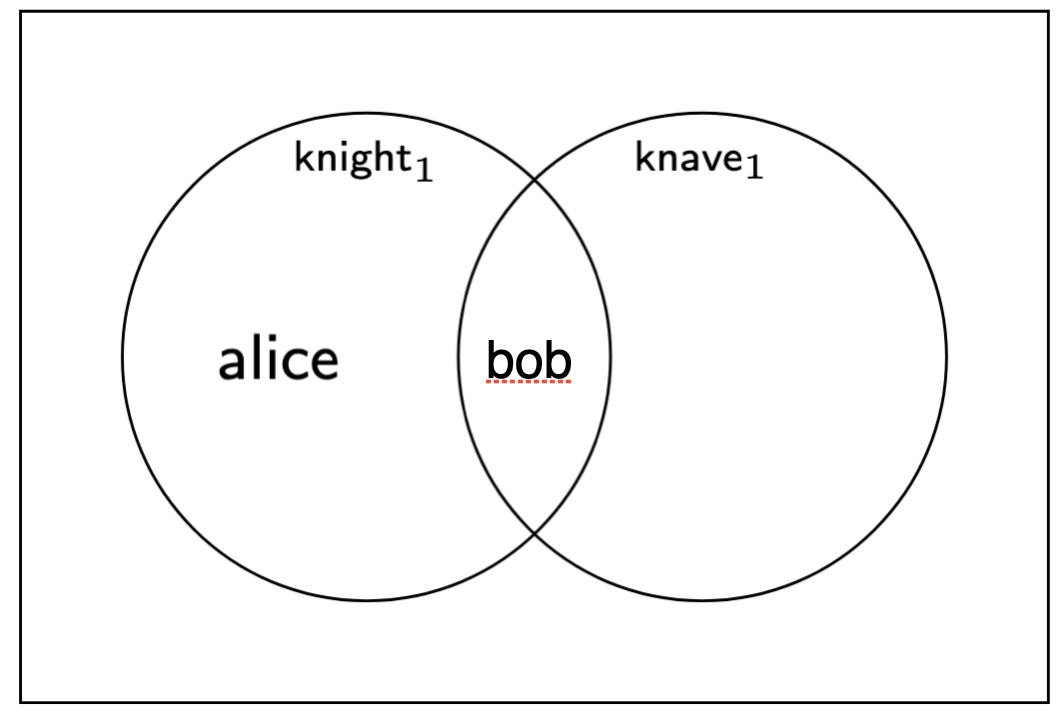
\includegraphics[width=\textwidth]{model7.png}

	\end{minipage}
	\hspace{0.5cm}
	\begin{minipage}[b]{0.45\linewidth}
		\centering
		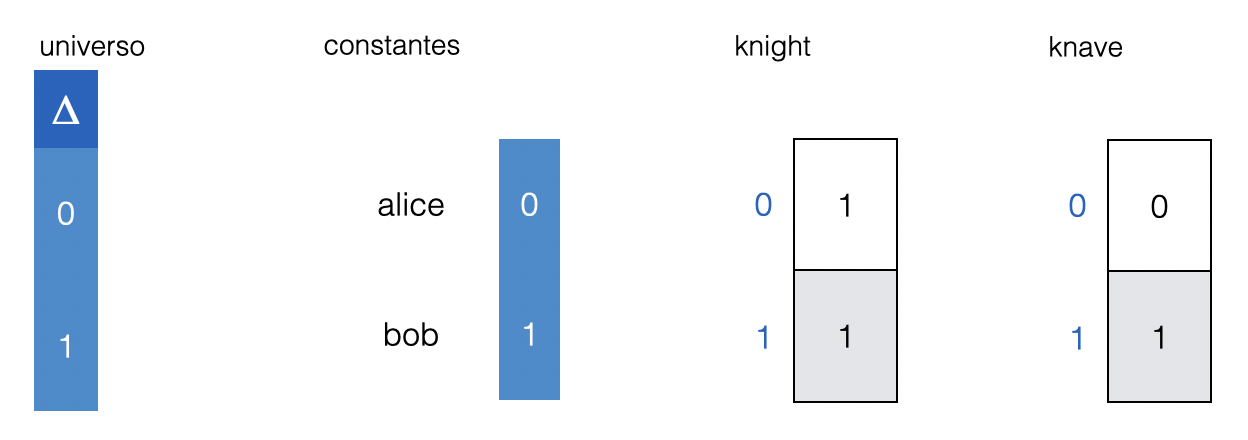
\includegraphics[width=\textwidth]{model6.png}
		%\caption{}
		%\label{}
	\end{minipage}
\end{figure}

{\bf valuación}
$\eval{\lnot(\exists x :: \knight(x) \land \knave(x))} = 0$

{\bf justificación}

$
	\begin{nd}
		\hypo{}{\eval{\lnot(\exists x :: \knight(x) \land \knave(x))}}
		\have{}{1- \eval{(\exists x :: \knight(x) \land \knave(x))}}
		\open
		\hypo{}{\eval{(\exists x :: \knight(x) \land \knave(x))}}
		\have{}{\max}
		\open
		\hypo{}{\eval{\knight(x) \land \knave(x)} \text{~~cuando $x=1$}}
		\have{}{\min(\eval{\knight(x)},\eval{\knave(x)})}
		\open
		\hypo{}{\eval{\knight(x)}}
		\have{}{1}
		\close
		\have{}{\eval{\knave(x)}}
		\have{}{1}
		\close
		\have{}{1}
		\close
		\have{}{1-1}
		\have{}{0}
	\end{nd}
$
\newpage

Un modelo para la fórmula $\forall p :: \ambassador(p) \to (\exists c :: \sentto(p,c)))$


\begin{figure}[t]
	\centering
	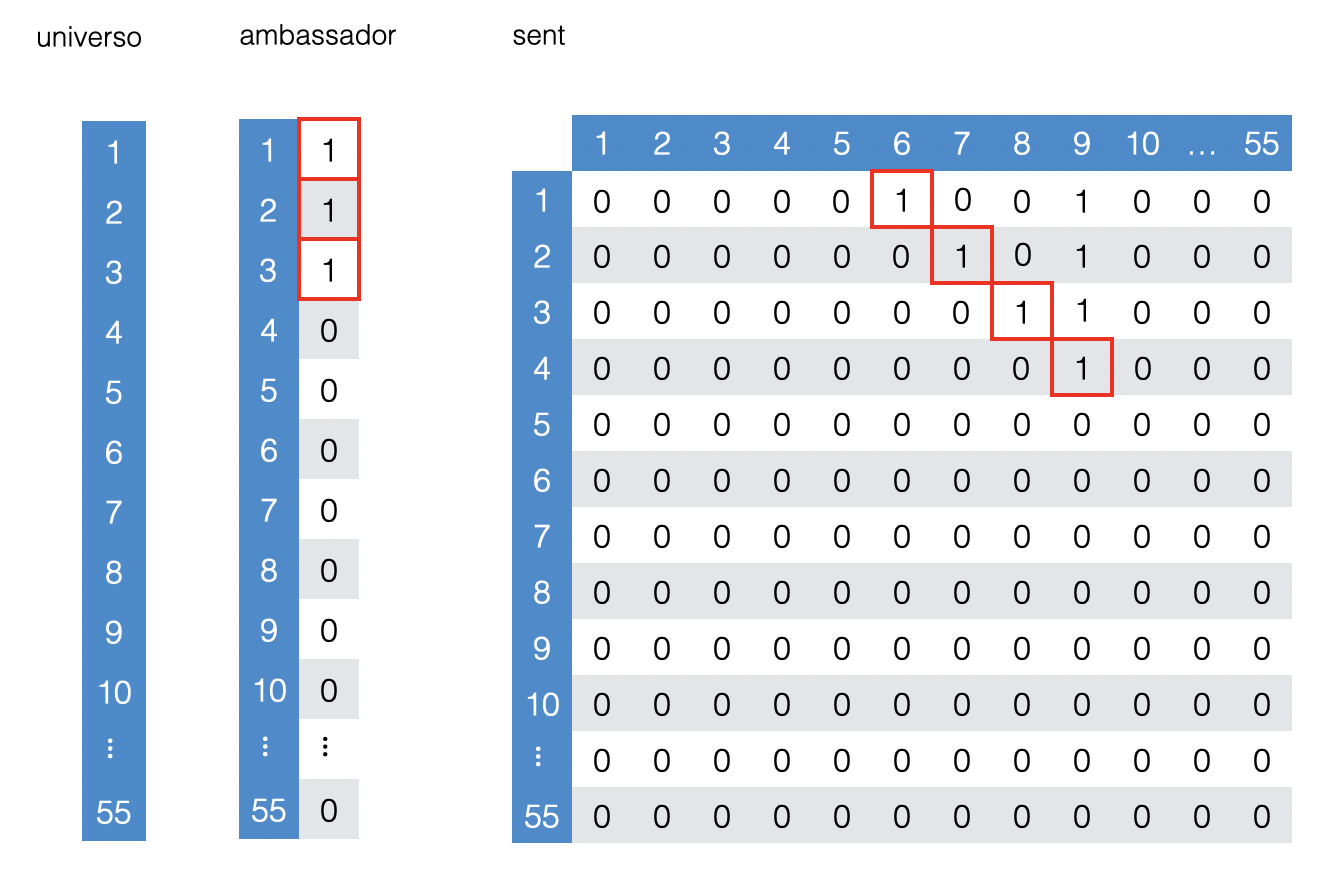
\includegraphics[scale=.45]{model8.png}

\end{figure}
{\bf valuación}
$\eval{(\forall p :: \ambassador(p) \to (\exists c :: \sentto(p,c)))} = 1$

{\bf justificación}


$
	\begin{nd}
		\hypo{}{\eval{(\forall p :: \ambassador(p) \to (\exists c :: \sentto(p,c)))}}
		\have{}{\min}
		\open
		\hypo{}{\eval{\ambassador(p) \to (\exists c :: \sentto(p,c))}~~\text{cuando $p = 1$}}
		\have{}{\max(1-\eval{\ambassador(p)}, \eval{(\exists c :: \sentto(p,c))})}
		\open
		\hypo{}{\eval{\ambassador(p)}}
		\have{}{1}
		\close
		\have{}{\eval{(\exists c :: \sentto(p,c))}}
		\have{}{\max}
		\open
		\hypo{}{\eval{\sentto(p,c)}~~\text{cuando $c = 6$}}
		\have{}{1}
		\close
		\have{}{1}
		\close
		\open
		\hypo{}{\eval{\ambassador(p) \to (\exists c :: \sentto(p,c))}~~\text{cuando $p = 2$}}
		\have{}{\max(1-\eval{\ambassador(p)}, \eval{(\exists c :: \sentto(p,c))})}
		\open
		\hypo{}{\eval{\ambassador(p)}}
		\have{}{1}
		\close
		\have{}{\eval{(\exists c :: \sentto(p,c))}}
		\have{}{\max}
		\open
		\hypo{}{\eval{\sentto(p,c)}~~\text{cuando $c = 7$}}
		\have{}{1}
		\close
		\have{}{1}
		\close
		\open
		\hypo{}{\eval{\ambassador(p) \to (\exists c :: \sentto(p,c))}~~\text{cuando $p = 3$}}
		\have{}{\max(1-\eval{\ambassador(p)}, \eval{(\exists c :: \sentto(p,c))})}
		\open
		\hypo{}{\eval{\ambassador(p)}}
		\have{}{1}
		\close
		\have{}{\eval{(\exists c :: \sentto(p,c))}}
		\have{}{\max}
		\open
		\hypo{}{\eval{\sentto(p,c)}~~\text{cuando $c = 8$}}
		\have{}{1}
		\close
		\have{}{1}
		\close
		\open
		\hypo{}{\eval{\ambassador(p) \to (\exists c :: \sentto(p,c))}~~\text{cuando $p \in [4,55]$}}
		\have{}{\max(1-\eval{\ambassador(p)}, \eval{(\exists c :: \sentto(p,c))})}
		\open
		\hypo{}{\eval{\ambassador(p)}}
		\have{}{0}
		\close
		\have{}{1}
		\close
		\have{}{1}
	\end{nd}
$

\newpage
$
	\begin{nd}
		\hypo{}{\eval{(\forall p :: \ambassador(p) \to (\exists c :: \sentto(p,c)))}}
		\have{}{\min}
		\open
		\hypo{}{\eval{\ambassador(p) \to (\exists c :: \sentto(p,c))}~~\text{cuando $p \in [1,2,3]$}}
		\have{}{\max(1-\eval{\ambassador(p)}, \eval{(\exists c :: \sentto(p,c))})}
		\open
		\hypo{}{\eval{\ambassador(p)}}
		\have{}{1}
		\close
		\have{}{\eval{(\exists c :: \sentto(p,c))}}
		\have{}{\max}
		\open
		\hypo{}{\eval{\sentto(p,c)}~~\text{cuando $c = 9$}}
		\have{}{1}
		\close
		\have{}{1}
		\close
		\open
		\hypo{}{\eval{\ambassador(p) \to (\exists c :: \sentto(p,c))}~~\text{cuando $p \in [4,55]$}}
		\have{}{\max(1-\eval{\ambassador(p)}, \eval{(\exists c :: \sentto(p,c))})}
		\open
		\hypo{}{\eval{\ambassador(p)}}
		\have{}{0}
		\close
		\have{}{1}
		\close
		\have{}{1}
	\end{nd}
$


%$(\forall p :: \ambassador(p)) \to (\exists c :: \sentto(p,c))$

Analizar la siguiente fórmula:
$(\forall p :: (\exists c :: \ambassador(p) \to \sentto(p,c)))$

\newpage

y si invertimos el orden de los cuantificadores?

$(\exists c :: (\forall p :: \ambassador(p) \to \sentto(p,c)))$


$
	\begin{nd}
		\hypo{}{\eval{(\exists c :: (\forall p :: \ambassador(p) \to \sentto(p,c)))}}
		\have{}{\max}
		\open
		\hypo{}{\eval{(\forall p :: \ambassador(p) \to \sentto(p,c))}~~\text{cuando $c = ??$}}
		\have{}{\min}
		\open
		\hypo{}{\eval{\ambassador(p) \to \sentto(p,c)}~~\text{cuando $p = ??$}}
		\have{}{??}
		\close
		\open
		\hypo{}{\eval{\ambassador(p) \to \sentto(p,c)}~~\text{cuando $p = [4,55]$}}
		\have{}{1}
		\close
		\have{}{??}
		\close
		\have{}{??}
	\end{nd}
$

\end{document}
